\section{Przekazywanie informacji o świecie w grach (Bartosz Strzelecki)}\label{chap:dbd}
Systemy przekazywania graczowi informacji o świecie są nieocenioną pomocą w kształtowaniu dynamiki i dostarczaniu kluczowych informacji.
Jest to podstawowy element rozgrywki, pozwalający na dynamiczne podejmowanie decyzji oraz na koordynację działań w grach wieloosobowych.

W grze Dead by Daylight mechanika widzenia przez przeszkody jest istotnym elementem rozgrywki, który
zapewnia dodatkową warstwę strategii. Polega na wyświetlaniu reprezentacji odległych celów, przedmiotów i przeciwników
zakrytych przez przeszkody. Ta zdolność odgrywa kluczową rolę dla obu stron konfliktu.

W przypadku ocalałych ta mechanika jest dostępna dzięki atutom i przedmiotom. Mechanika ujawnia lokalizację celów oraz
innych ocalałych pozwalając na koordynację i opracowanie strategii wspólnych działań.

I odwrotnie, zdolność zabójcy do widzenia aury jest kluczowa dla jego mechaniki rozgrywki.
Aury umożliwiają im śledzenie ocalałych, zwłaszcza gdy korzystają z ich unikalnych mocy lub specyficznych atutów. 
Mechanika ta zwiększa napięcie, ponieważ ocalali muszą zachować czujność i strategiczne podejście, 
aby uniknąć pola widzenia zabójcy lub zakłócić ich zdolność czytania aury, aby uciec i osiągnąć cele.

\begin{figure}[h]
\centering
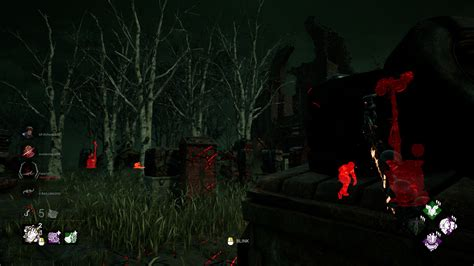
\includegraphics[width=0.6\textwidth]{images/aura}
\caption{Przykładowe elementy widzenia przez horyzont w grze Dead by Daylight.}
\end{figure}

Ogólnie rzecz biorąc, mechanika aury w Dead by Daylight służy jako podstawowy element rozgrywki,
który równoważy wymianę informacji między ocalałymi a zabójcami, znacząco przyczyniając się do atmosfery napięcia i strategii w grze.

\begin{figure}[h]
\centering
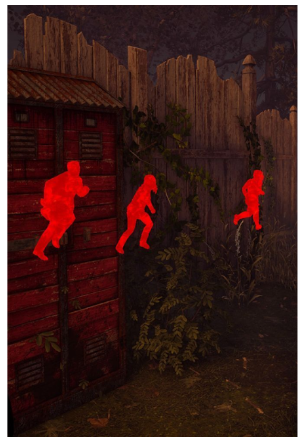
\includegraphics[width=0.6\textwidth]{images/dbd}
\caption{Przykładowy efekt aury w grze Dead by Daylight.}
\end{figure}
